\section{Results}
\subsection{The DeepPBS Framework}
The DeepPBS framework is illustrated in Fig. 1. Input to DeepPBS (Fig. 1a) is composed of one protein-DNA complex structure, with one or more protein chains bound to a DNA double helix. Potential sources for such structures include experimental data (for example, PDB\citep{berman2000protein}), molecular simulation snapshots or designed complexes. DeepPBS processes the structure as a bipartite graph with distinct spatial graph representations for protein and DNA components. The protein graph is an atom-based graph, with heavy atoms as vertices. Several features are computed on these vertices (Fig. 1b). Further information on protein representation and feature computation is available in Methods. We represent DNA as a symmetrized helix (sym-helix), as detailed in Methods. This representation removes any sequence identity that the DNA possesses, while preserving the shape of the double helix \citep{rohs2009role}. Optionally, DNA sequence information can be reintroduced as a feature on the sym-helix points.
\par
DeepPBS performs a series of spatial graph convolutions on the protein graph to aggregate atomic neighborhood information (Fig. 1d). The next crucial component of DeepPBS consists of a set of bipartite geometric convolutions applied from the protein graph to the sym-helix (Fig. 1d). Specific chemical interactions (for example, hydrogen bonds) depend on both location and orientation \citep{Helene1977}. DeepPBS learns how the geometric orientation of the sym-helix points is associated with the orientations and chemistry of neighboring protein residues. Four distinct bipartite convolutions are employed for the sym-helix points, corresponding to the major groove, the minor groove and the phosphate and sugar moieties. Major and minor groove convolutions are referred to as ‘groove readout’. This term was chosen over the term ‘base readout’ due to the removal of base identity in the sym-helix. Phosphate and sugar moiety convolutions, combined with DNA shape information, form the ‘shape readout’ (Fig. 1e). The ‘groove readout’ and ‘shape readout’ factors collaboratively determine binding specificity to varying extents for different protein families. At this point, the sym-helix representation enables a straightforward flattening of aggregated features on the three-dimensional sym-helix to the one-dimensional (1D) base pair-level features. By adding DNA shape information and implementing 1D convolutional neural network and prediction layers (Fig. 1e), DeepPBS ultimately predicts binding specificity (Fig. 1f). Further architectural details are described in Supplementary Section 5.
\par
Lack of an existing published standard dataset for predicting binding specificity across protein families from protein-DNA complex structure data made it necessary for us to build a dataset for cross-validation and benchmarking. Details of this process can be found in Methods.

\begin{center}
    \begin{figure}
    \makebox[\textwidth]{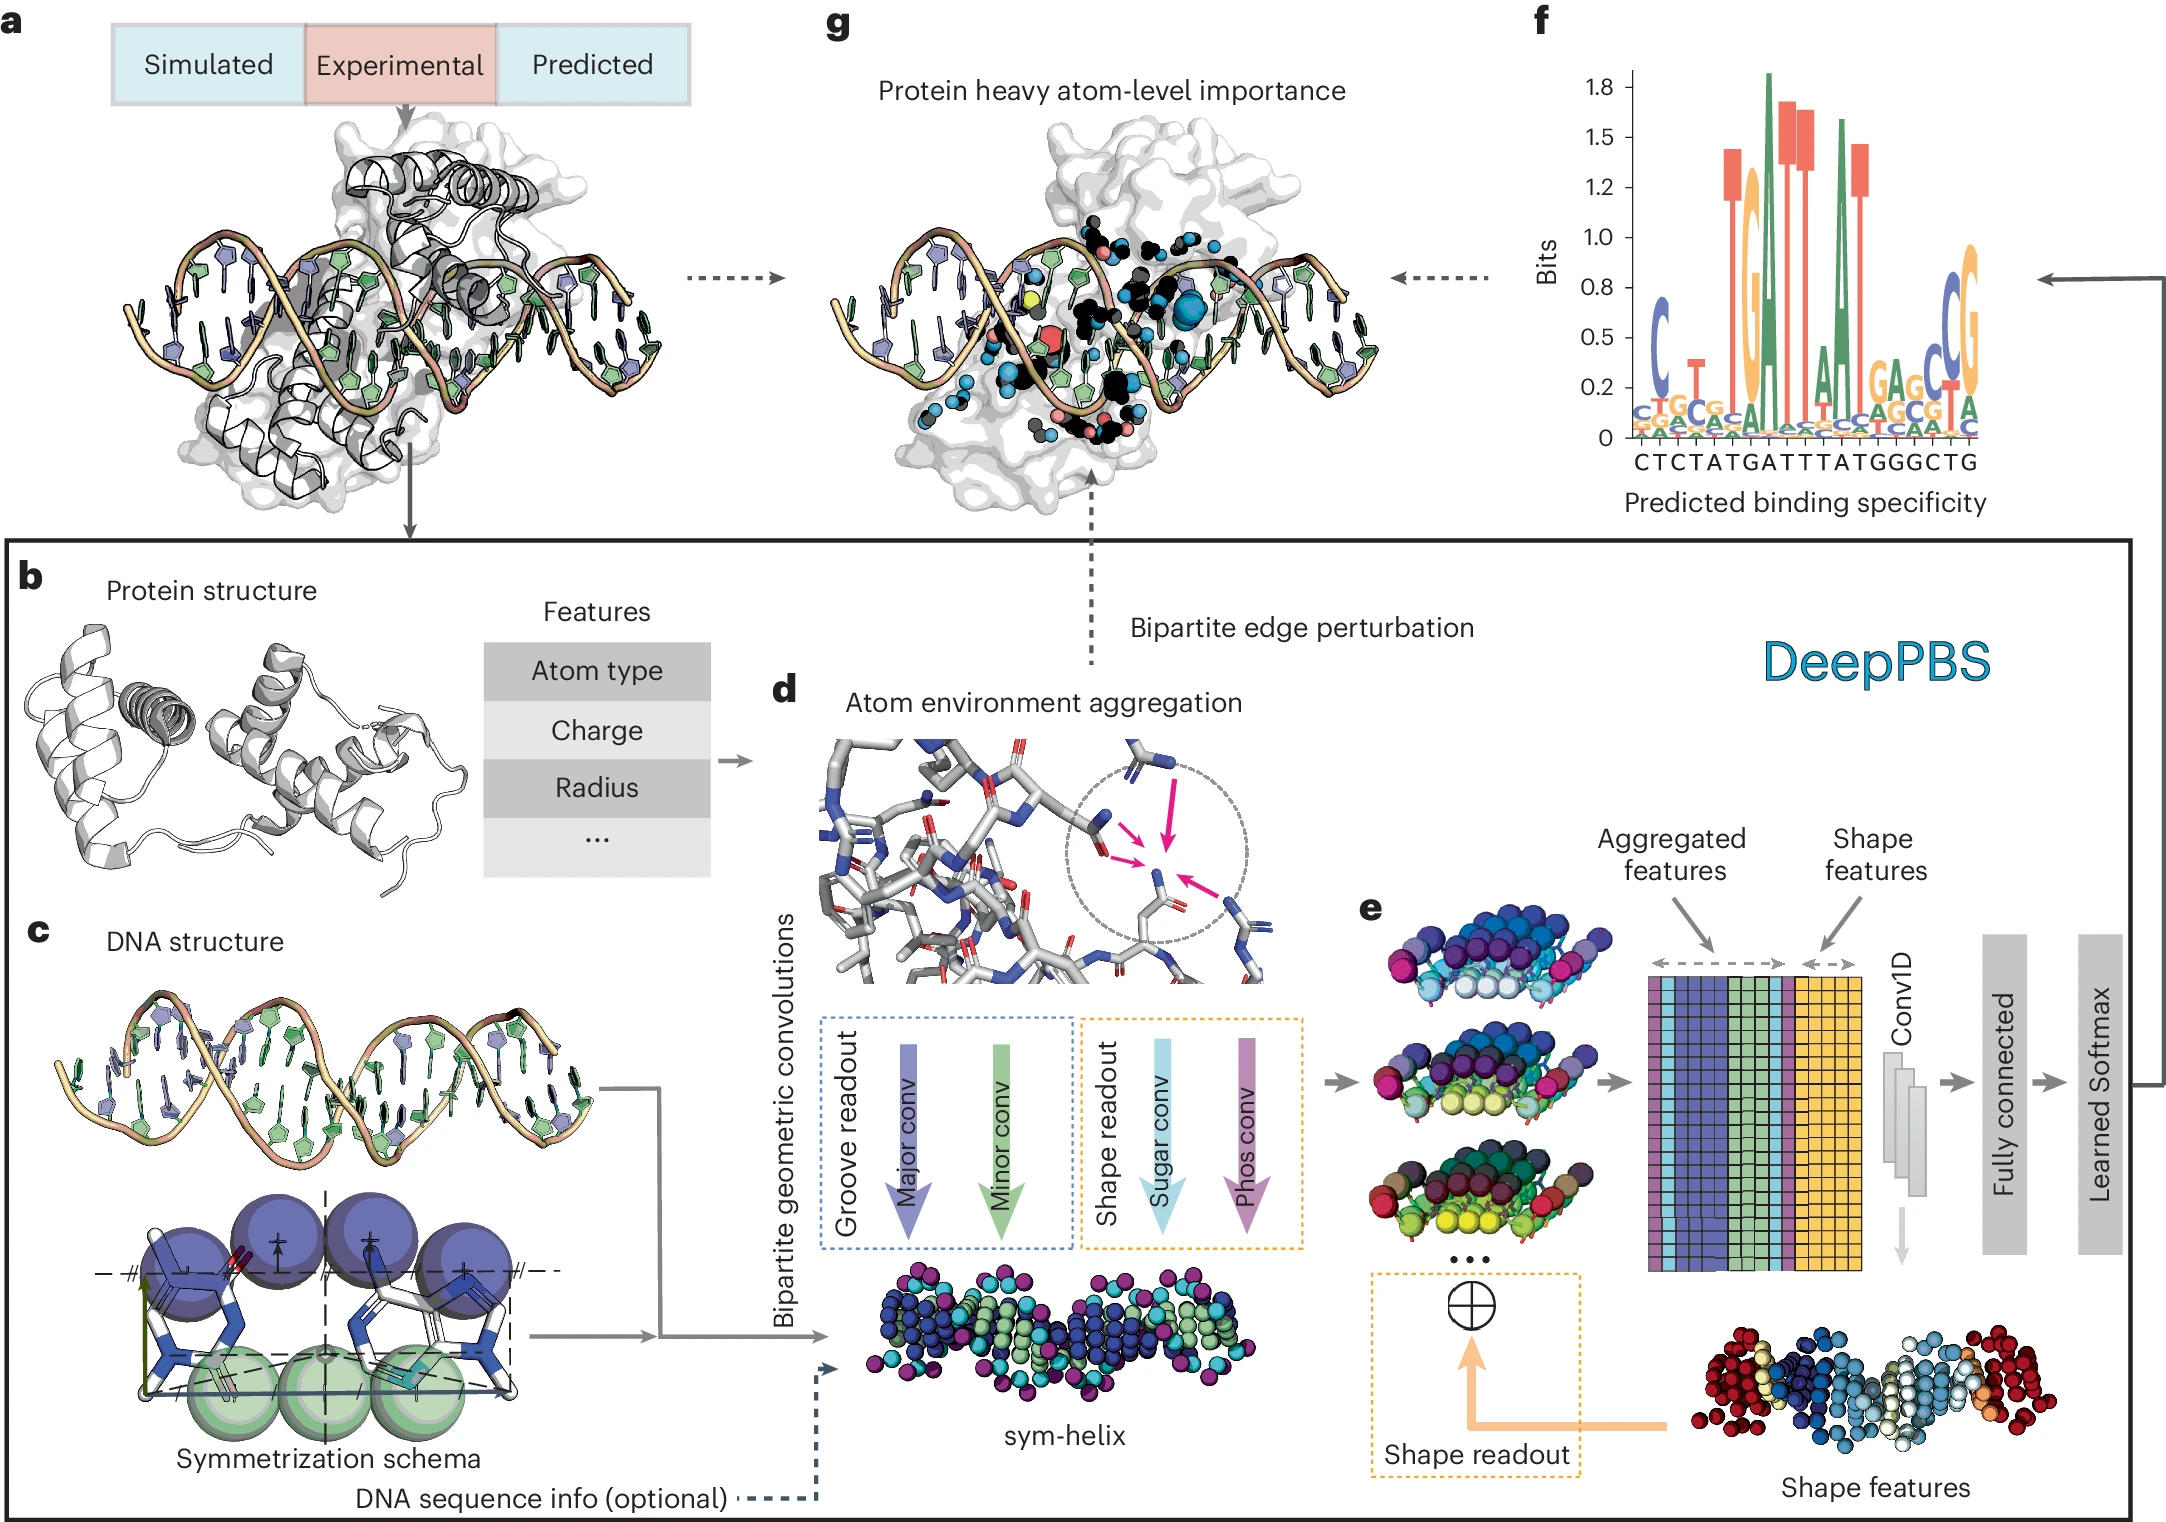
\includegraphics[width=0.8\paperwidth]{./pdnafigs/fig1.png}}
 % archetecture.png: 1149x508 px, 72dpi, 40.53x17.92 cm, bb=0 0 1149 508
        \caption[Computational cost of training RVAgene]{\textbf{Training RVAgene is reasonably scalable on CPU and even more so using hardware acceleration through GPU.} ({\bf A}) Time cost of training RVAgene for 100 epochs for datasets with varying number of genes and time points on CPU and GPU. ({\bf B}) Maximum memory utilized during training of the model on CPU an GPU for the cases in (A), inset plot: comparison of max memory used compared to DPGP for varying number of genes.}
  \label{fig:pdna1}
\end{figure}
\end{center}

\subsection{DeepPBS performance for experimentally determined structures}
The DeepPBS ensemble (Methods) was employed to evaluate model performance against a benchmark set, as outlined in Supplementary Section 1. The DeepPBS architecture allows models to be trained on two mechanisms: ‘groove readout’, which does not involve backbone convolutions and excludes shape information, and ‘shape readout’, which does not involve groove convolutions (Fig. 1d,e). Benchmark performances of DeepPBS (which performs both ‘groove readout’ and ‘shape readout’ modes combined) and these two variations are shown in Fig. 2a. The ‘groove readout’ version does better than the ‘shape readout’ version in terms of median performance, while the DeepPBS model improves upon either component in isolation (two-sided t-test P value <0.01; Fig. 2a). Pairwise t-test P values for these variations are available (Supplementary Data 1). A discussion of the outliers in Fig. 2a is provided in Supplementary Section 12.
\par
The dataset was constructed using experimentally determined structures; thus, the co-crystal structure-derived DNA sequence typically serves as a reasonable example of a bound sequence. As expected, integrating sequence information into the sym-helix points (‘DeepPBS with DNA SeqInfo’) enhanced performance (Fig. 2a), significantly closing the gap toward the inherent performance limit in the dataset. The inherent performance limit originates from the fact that for the same protein the binding specificity data presented by two databases \citep{Jaime2022, kulakovskiy2018hocomoco} used to create the dataset may disagree to some extent (Supplementary Fig. 1c). We computed the distribution of disagreement across all unique PWMs appearing in both databases (Supplementary Section 1). However, from both interpretability and design perspectives, particularly when the bound DNA sequence may not be representative, the ‘DeepPBS’ model is optimal due to its low sensitivity to the DNA sequence in the structure. This fact is evidenced by comparing performances of the ‘DeepPBS’ and ‘DeepPBS with DNA SeqInfo’ models in the context of the PWM-co-crystal-derived DNA alignment score (Supplementary Section 1). Compared with the line fit to the variation with DNA sequence information (slope $-0.44$ for root mean squared error (RMSE), slope $-0.62$ for mean absolute error (MAE); Supplementary Fig. 11), the slope of the line fit to the DeepPBS predictions was closer to zero (Fig. 2b and Supplementary Fig. 11).
\par
As an example, we show the DeepPBS ensemble prediction for the NF-$\kappa$B biological assembly from the benchmark dataset. Although the co-crystal structure-derived DNA sequence was not of the highest binding affinity, as indicated by experimental data from HOCOMOCO \citep{kulakovskiy2018hocomoco}, our prediction circumvented this issue, predicting a binding specificity that was more closely aligned with the experimental data (Supplementary Fig. 5d). Similar trends (Supplementary Fig. 5a-c) can be observed from cross-validation predictions by individual DeepPBS models (Methods). We also included example DeepPBS ensemble predictions (Supplementary Fig. 7) for structures in the PDB that correspond to specific interactions but do not have a PWM in the two binding specificity databases considered (Methods). In addition, example DeepPBS ensemble predictions (Supplementary Fig. 8) for structures of nonspecific protein-DNA binding (for example, SSO7D-DNA interaction \citep{Agback1998}) present in the PDB are presented. These predictions have notably lower information content compared with those in Supplementary Fig. 7.

\subsection{DeepPBS captures patterns of family-specific binding modes}
Abundances of different protein families in the benchmark set are described in Fig. 2c (Supplementary Fig. 5b for cross-validation set). Family annotations were obtained from the Database of Protein Families (PFAM) \citep{Mistry2021}. The dataset encompasses a wide range of DNA-binding protein families. Performance of DeepPBS for various protein families provides several key insights. DeepPBS showed reasonable generalizability across protein families, performing well even for families with relatively fewer structures (Fig. 2d and Supplementary Fig. 5c), such as heat shock factor proteins. This observation suggests that the model is learning the underlying mechanisms of protein-DNA binding rather than overfitting on family-specific patterns.
\par
Further validation is provided by comparing performances of the DeepPBS ‘groove readout’ and ‘shape readout’ models (Fig. 2d and Supplementary Fig. 5c). For families like zf-C2H2, zf-C4 the ‘shape readout’ model did not perform as well as the ‘groove readout’ model. This result aligns with the common understanding of the binding mechanism of these families. For example, zf-C2H2 uses zinc finger motifs to scan DNA for suitable base interactions, with minimal DNA bending or conformational change \citep{Persikov2011}. This binding mode makes the zf-C2H2 family a popular target of protein sequence-based binding specificity prediction and design \citep{Persikov2014, persikov2009predicting, aizenshtein2022deepzf, Yanover2011, Ichikawa2023}. Conversely, families like interferon-regulatory factor (IRF) proteins (Fig. 2d and Supplementary Fig. 5c) and T-box proteins (Supplementary Fig. 5c) showed higher performances for the ‘shape readout’ model, consistent with their known binding mechanisms that involve significant conformational changes\citep{Stirnimann2010, Escalante1998}. For families such as homeodomain (HD) and forkhead (Fig. 2d and Supplementary Fig. 5c), the DeepPBS model outperformed both the ‘groove readout’ and ‘shape readout’ components. This result suggests that the network captures complex higher-order relationships of these components. Pairwise P values for the three readout variations for Fig. 2d and Supplementary Fig. 5c are available in Supplementary Data 1.

\begin{center}
    \begin{figure}
    \makebox[\textwidth]{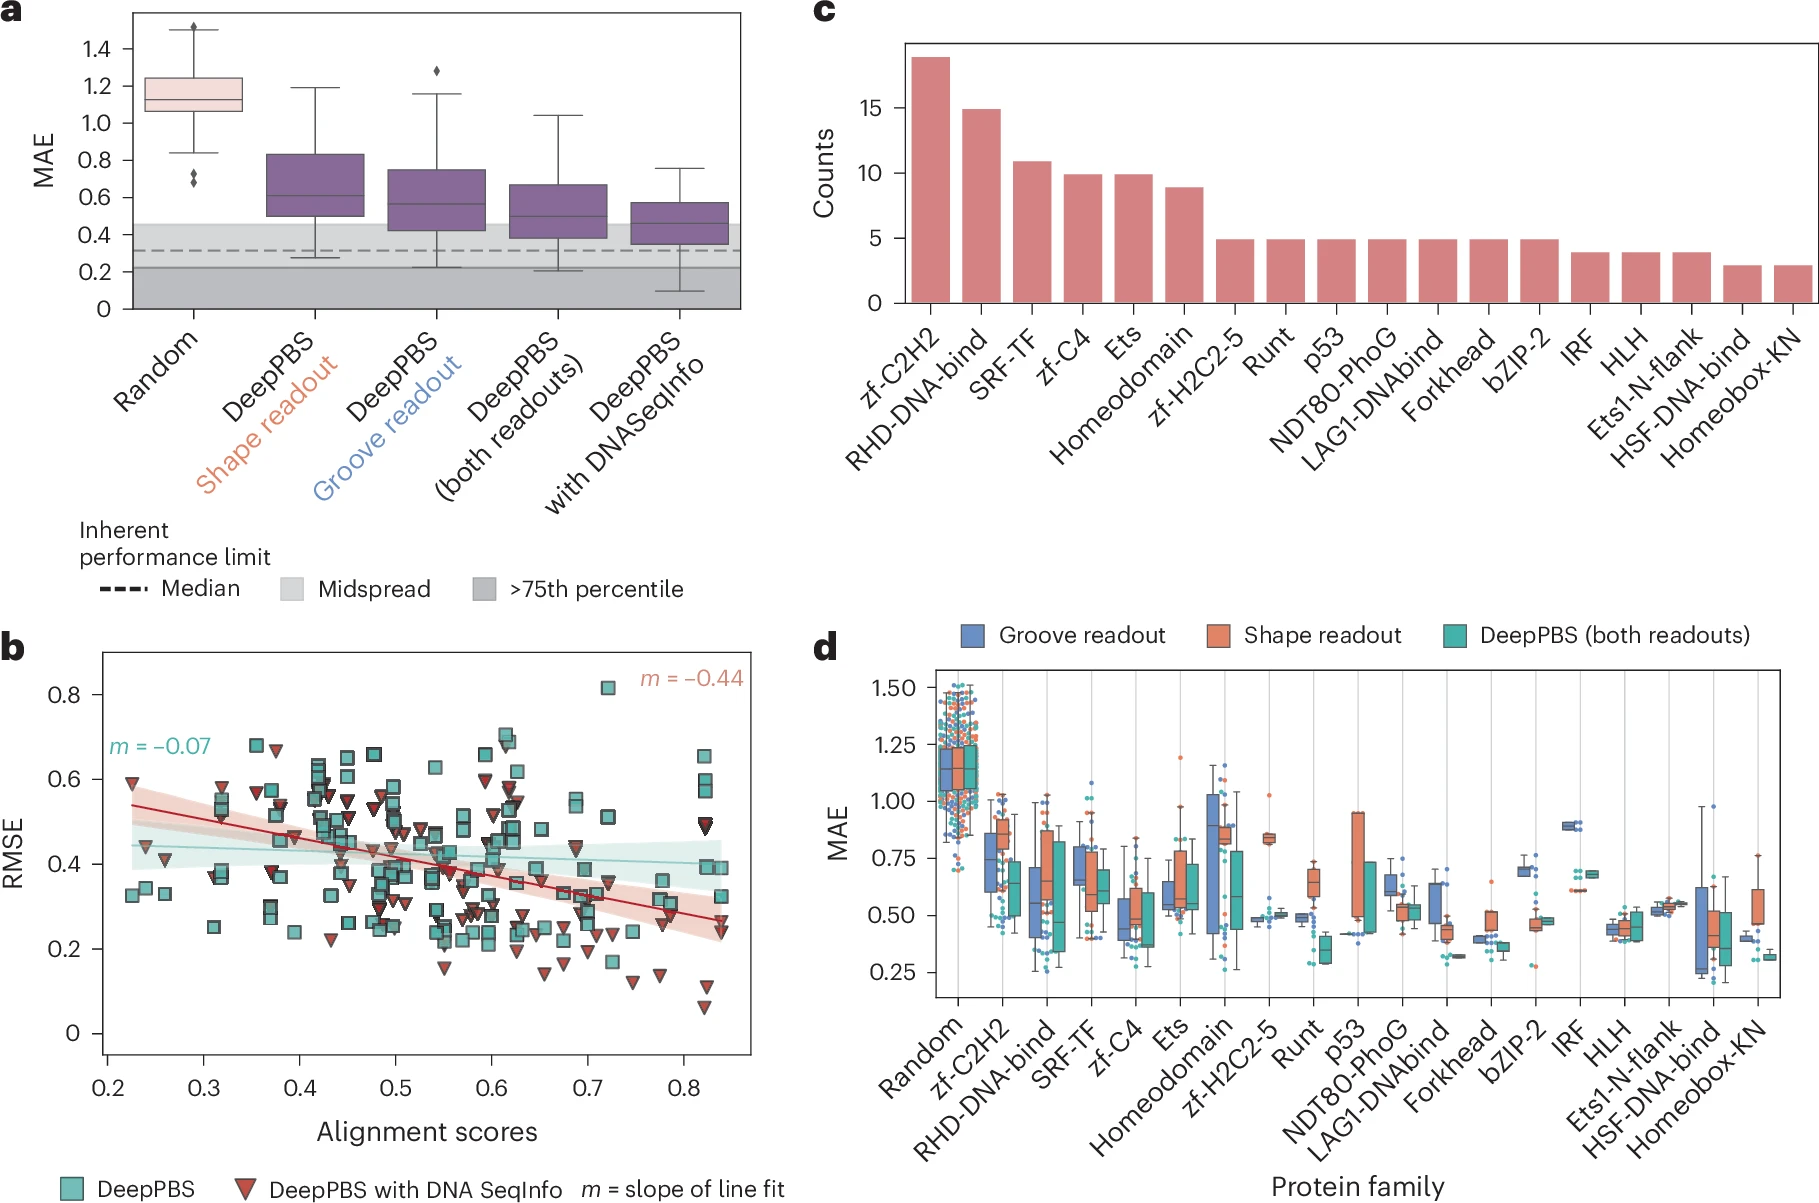
\includegraphics[width=0.8\paperwidth]{./pdnafigs/fig2.png}}
 % archetecture.png: 1149x508 px, 72dpi, 40.53x17.92 cm, bb=0 0 1149 508
        \caption[Computational cost of training RVAgene]{\textbf{Training RVAgene is reasonably scalable on CPU and even more so using hardware acceleration through GPU.} ({\bf A}) Time cost of training RVAgene for 100 epochs for datasets with varying number of genes and time points on CPU and GPU. ({\bf B}) Maximum memory utilized during training of the model on CPU an GPU for the cases in (A), inset plot: comparison of max memory used compared to DPGP for varying number of genes.}
  \label{fig:pdna2}
\end{figure}
\end{center}

\subsection{Application to in silico-predicted protein–DNA complexes}
The DeepPBS framework is not limited to experimental structures. Recent advances in scalable structural prediction approaches, driven by artificial intelligence26,28, offer unprecedented potential. Specifically, models like RFNA \citep{baek2024na} and MELD-DNA \citep{Esmaeeli2023} can be used to predict the structures of protein-DNA complexes from sequence. Such prediction algorithms have paved the way for DeepPBS to be applicable to proteins that lack experimental DNA-bound structure data.
\par
We suggest one potential approach for working with predictive structures in DeepPBS. First, we make an initial guess for the DNA (IG DNA) sequence bound to each protein of interest based on the corresponding protein family. Then, we use RFNA to predict the protein-DNA complex structure, followed by DeepPBS to predict binding specificity. We demonstrate this process (Fig. 3a-c) for three proteins classified as basic helix-loop-helix (bHLH) in JASPAR \citep{Jaime2022}. In all three cases, the PDB lacked experimental protein-DNA complex structures. The IG DNA (Supplementary Section 8) has an enhancer box motif (‘CACGTG’) in the center, which is known \citep{demartin2021} to be a bHLH family target. The first example (UniProt Q4H376; Fig. 3a) is a Max homodimer, for which DeepPBS predicted a specificity closely mirroring that of the IG DNA. The second example (TCF21 dimer, O43680) was more complicated; the central ‘CACGTG’ motif in the IG DNA was erroneously assumed, yet DeepPBS successfully predicted the correct motif as ‘CATATG’ (Fig. 3b). The third example (Fig. 3c, protein OJ1581$\_$H09.2, Q6H878) does not conform to any enhancer box motif. Nevertheless, DeepPBS predicted a binding specificity closely mirroring the experimental data (Fig. 3c).
\par
We ran the DeepPBS pipeline for full-length UniProt protein sequences, each with a unique JASPAR entry and no experimental structure for the complex, across three different families (Supplementary Section 8): bZIP, bHLH and HD families. DeepPBS predictions based on RFNA-predicted structures exhibited an improved MAE (that is, closer to experimental data) compared with the IG DNA baseline (Fig. 3d). An application of DeepPBS to a MELD-DNA-predicted complex of the mouse CREB1 protein is demonstrated in Supplementary Fig. 9b. Thus, DeepPBS can take predicted structures from suboptimal DNA sequences and predict binding specificity close to experimental data.
\par
We next explored whether DeepPBS prediction could be used as feedback (in a loop) to enhance modeling of the protein complex (and, subsequently, improve DeepPBS prediction). We demonstrated this process for the human TGIF2LY protein (UniProt ID Q8IUE0, unstructured region trimmed; Supplementary Section 8) in Fig. 3e. In round 1, we applied RFNA to this protein sequence alongside the IG DNA sequence for the HD family and then used the predicted complexes as input for DeepPBS. For IG DNA position T15 (Fig. 3e, round 1), DeepPBS predicted a strong preference for G. In the round 1 RFNA output, Arg57 and T15 were involved in one hydrogen bond (H-bond) and one van der Waals interaction. These interactions are theoretically weaker than the possible bidentate H-bonds between a G and Arg57. In round 2, we altered the RFNA input by taking the argmax (the most preferred sequence) from the DeepPBS output (Fig. 3e, round 2). The subsequently folded structure reflected a more robust bidentate H-bond interaction between G15 and Arg57, with the DeepPBS prediction more closely aligning with the experimental data (note positions (round 2) A18, G19 and T14, corresponding to positions 4-6 in MA1572.1; Fig. 3e).
\par
We repeated this DeepPBS prediction process for a total of seven rounds, for the set of HD monomer sequences (Supplementary Section 8). The RFNA-predicted confidence metric (predicted local distance difference test (pLDDT), LDDT \citep{Mariani2013} reflects similarity between the predicted and reference structure for a complex; Supplementary Section 8) improved over these rounds (Fig. 3f). To independently evaluate structure quality, we calculated the molecular mechanics and Poisson-Boltzmann surface area \citep{Genheden2015} binding energy (Supplementary Section 8). From round 1 to round 3+, the number of stable structures (binding energy $kJ/mol$) increased (Supplementary Fig. 9c), while their binding energy distributions shifted toward lower values (Supplementary Fig. 9c). DeepPBS performance improved across the five rounds (Supplementary Fig. 9a). We also refolded the benchmark set datapoints via RFNA (Supplementary Section 8) and compared (for the full processable set ($n=98$) and a high-confidence set, pLDDT $>$0.9, $n=31$) the performances with the equivalent performance obtained for the experimental structures (Fig. 3g). There is a drop in performance. We can expect that it will improve when future models for structure prediction become available.
\par
The DeepPBS approach for predicting binding specificity fundamentally differs from that of existing methods, which predict binding specificity solely on the basis of protein sequence information. As a result, comparisons with existing family-specific methods that operate exclusively on protein sequence are unfeasible. However, in conjunction with a complex structure prediction method, we can start from protein sequence information alone and predict binding specificity using DeepPBS. This process can be compared with the recent HD family-specific method, rCLAMPS \citep{Wetzel2022} (Supplementary Section 8). rCLAMPS can predict core 6-mer binding specificities for monomer HD proteins. A comprehensive overview of performances is shown in Fig. 3h. For different significant portions of the data, DeepPBS and rCLAMPS outperformed each other. DeepPBS outperformed rCLAMPS where the pLDDT scores were higher (Fig. 3i). Thus, the DeepPBS pipeline is comparable to rCLAMPS, while having broader applicability across families and biological assemblies as well as not being limited to predicting the DNA core binding region.

\begin{center}
    \begin{figure}
    \makebox[\textwidth]{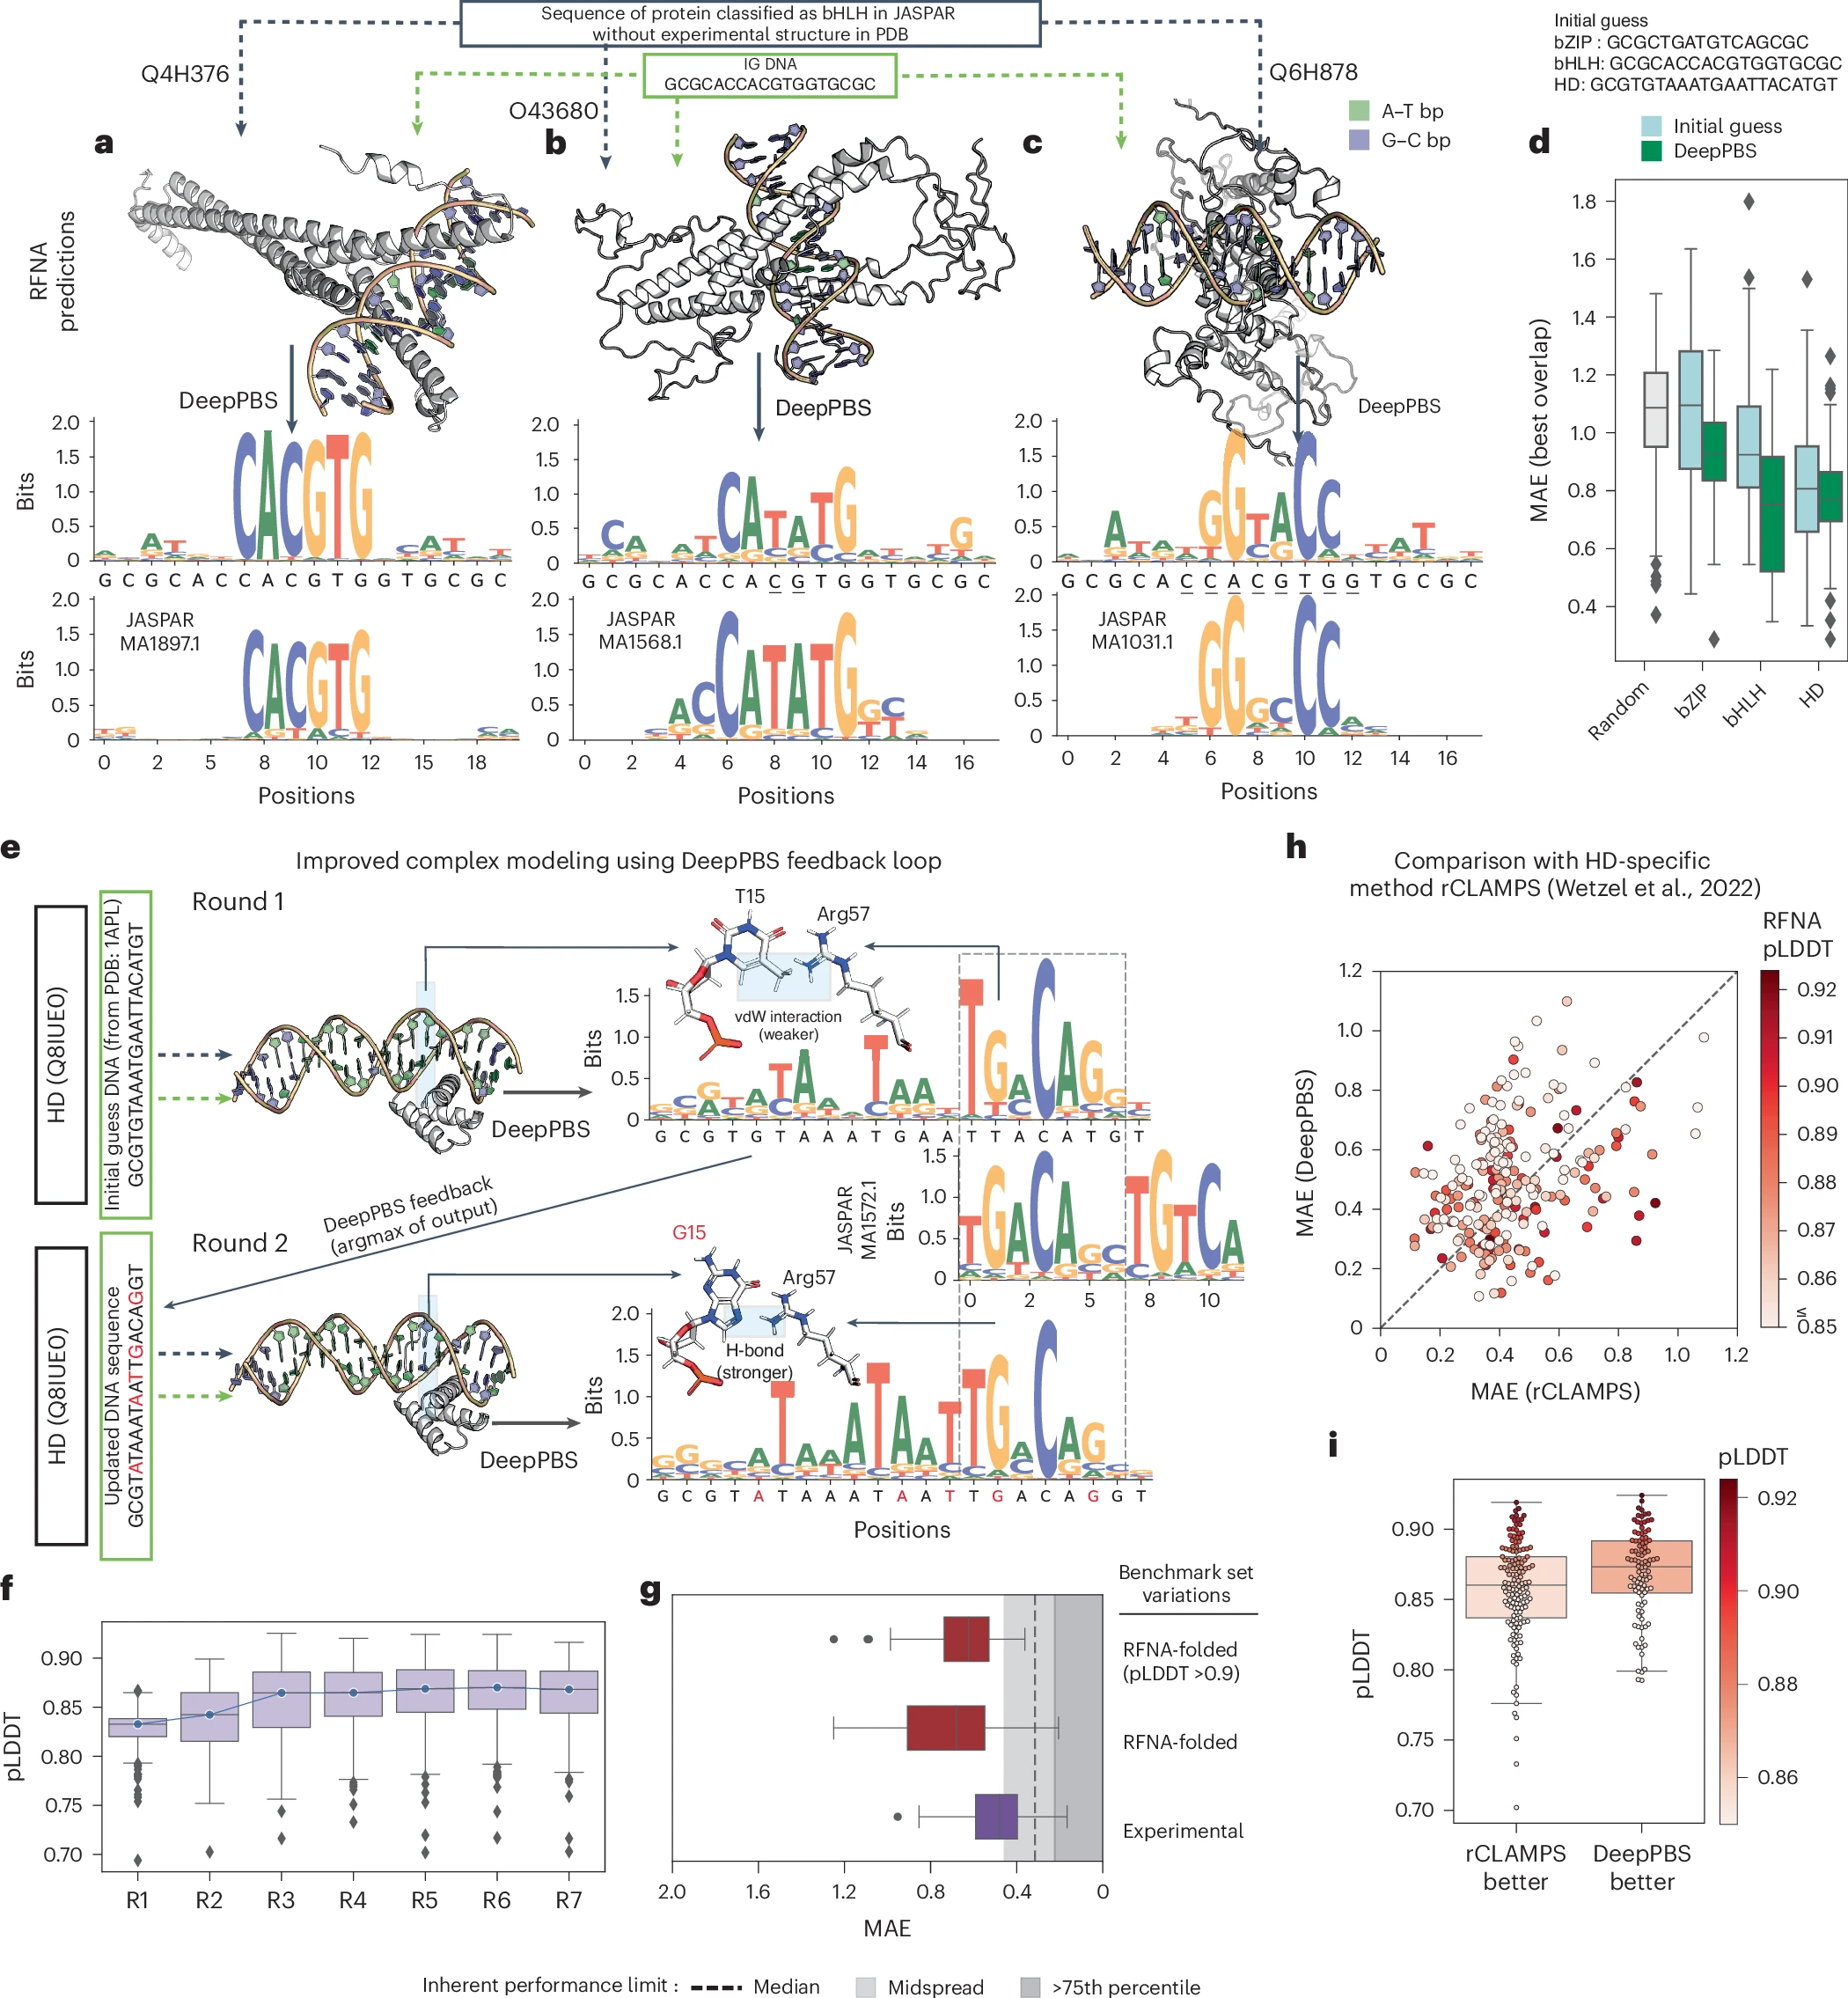
\includegraphics[width=0.8\paperwidth]{./pdnafigs/fig3.png}}
 % archetecture.png: 1149x508 px, 72dpi, 40.53x17.92 cm, bb=0 0 1149 508
        \caption[Computational cost of training RVAgene]{\textbf{Training RVAgene is reasonably scalable on CPU and even more so using hardware acceleration through GPU.} ({\bf A}) Time cost of training RVAgene for 100 epochs for datasets with varying number of genes and time points on CPU and GPU. ({\bf B}) Maximum memory utilized during training of the model on CPU an GPU for the cases in (A), inset plot: comparison of max memory used compared to DPGP for varying number of genes.}
  \label{fig:pdna3}
\end{figure}
\end{center}

\subsection{Assessing protein residue importance at p53-DNA interface}
The DeepPBS architecture permits intentional activation or deactivation of specific edges in the bipartite geometric convolution stage (Fig. 1d and Supplementary Fig. 4). Perturbing a set of edges in this manner will alter the network-predicted result. The mean absolute difference between the original and altered prediction can be used (with proper normalization) as a quantification of the impact of the perturbed set of edges in determining binding specificity (Fig. 1g, Supplementary Fig. 4 and Methods).
\par
We present results for perturbing edge sets for individual protein heavy atoms, which can also be aggregated to compute residue-level importance. As an example, we examined the protein-DNA interface of p53 (PDB ID: 3Q05), a protein crucial for regulating cancer development and cell apoptosis \citep{Joerger2008}. The tumor suppressor p53 binds to DNA as a tetramer with two symmetric protein-DNA interfaces \citep{Kitayner2010, Petty2011}. We show the RI scores (with min-max normalization applied) calculated for heavy atoms within $5\AA$ of the sym-helix (Fig. 4a). Sphere sizes in Fig. 4a denote computed RI scores, with the largest being 1 and smallest 0. Lys120 \citep{Kitayner2006} is involved in both groove readout (H-bond with G) and shape readout-based binding specificity (H-bond with backbone phosphate) (Fig. 4b). The network deems G-Arg280 \citep{Kitayner2006} bidentate H-bonds as another strong driver of binding specificity5 (Fig. 4c). Cys277 confers specificity through its thiol sulfur, accepting an H-bond in the major groove \citep{Kitayner2006} (Fig. 4d). Another important residue according to DeepPBS, Arg248 \citep{Barakat2011}, is present at the minor groove (Fig. 4e). This decision by the model is primarily based on the orientation of arginine relative to the sym-helix, which is devoid of DNA sequence information. Arg248 is attracted through enhanced negative electrostatic potential due to a narrowing of the minor groove where it binds \citep{Kitayner2010}. Among other residues in Fig. 4f, Ser241 is known \citep{Barakat2011} to be important for stabilizing Arg248. Ala276 (known for causing apoptosis upon mutation \citep{Reaz2013}) appears as another driver of specificity. This residue has been shown to be a driver of specificity via van der Waals contacts with the methyl group of T in the major groove\citep{Kitayner2006}. The binding specificity prediction of DeepPBS (Fig. 4g) aligns well with known binding patterns of p53, which follows the form RRRC(A/T)(A/T)GYYY (R denotes purine, and Y denotes pyrimidine). The interactions shown here are deemed \citep{Joerger2008, Vousden2009} as significant drivers of p53 binding.

\subsection{Comparison of residue-level importance with mutagenesis data}
We next asked whether DeepPBS-derived importance scores, which reflect the degree to which an interaction determines output binding specificity, can be considered as reliable and potentially physically significant. Although high-affinity interactions can be nonspecific \citep{Agback1998, Peterson2007}, interactions that contribute to high specificity would be expected to maximize binding affinity across different base pair possibilities. Therefore, the DeepPBS importance scores associated with these interactions should display some correlation with the corresponding binding affinities. We can test this hypothesis experimentally by using alanine scanning mutagenesis data (Supplementary Section 1). Sets of such experimental data have been made available through recent contributions\citep{Ovek2022} in the field. Utilizing these data \citep{Peng2018}, we applied suitable filtering for our context and calculated the log sum aggregated residue level importance scores using DeepPBS (Methods).
\par
A regression plot and Pearson’s correlation coefficient (PCC), as shown in Fig. 4h, illustrate the correspondence between computed values and experimental $\Delta\Delta G$ values for a diverse array of proteins and residues within the protein-DNA interface (Supplementary Table 1). The obtained PCC of 0.60 corroborates our hypothesis. It is noteworthy that the model was not trained to predict these values. These values were only obtained through perturbing the wild-type (WT) structures as input (Supplementary Fig. 4 and Supplementary Table 1). These results highlight the potential of DeepPBS as an economical guide for experimentalists who are selecting alanine scanning mutagenesis experiments to conduct at the protein-DNA interface.

\begin{center}
    \begin{figure}
    \makebox[\textwidth]{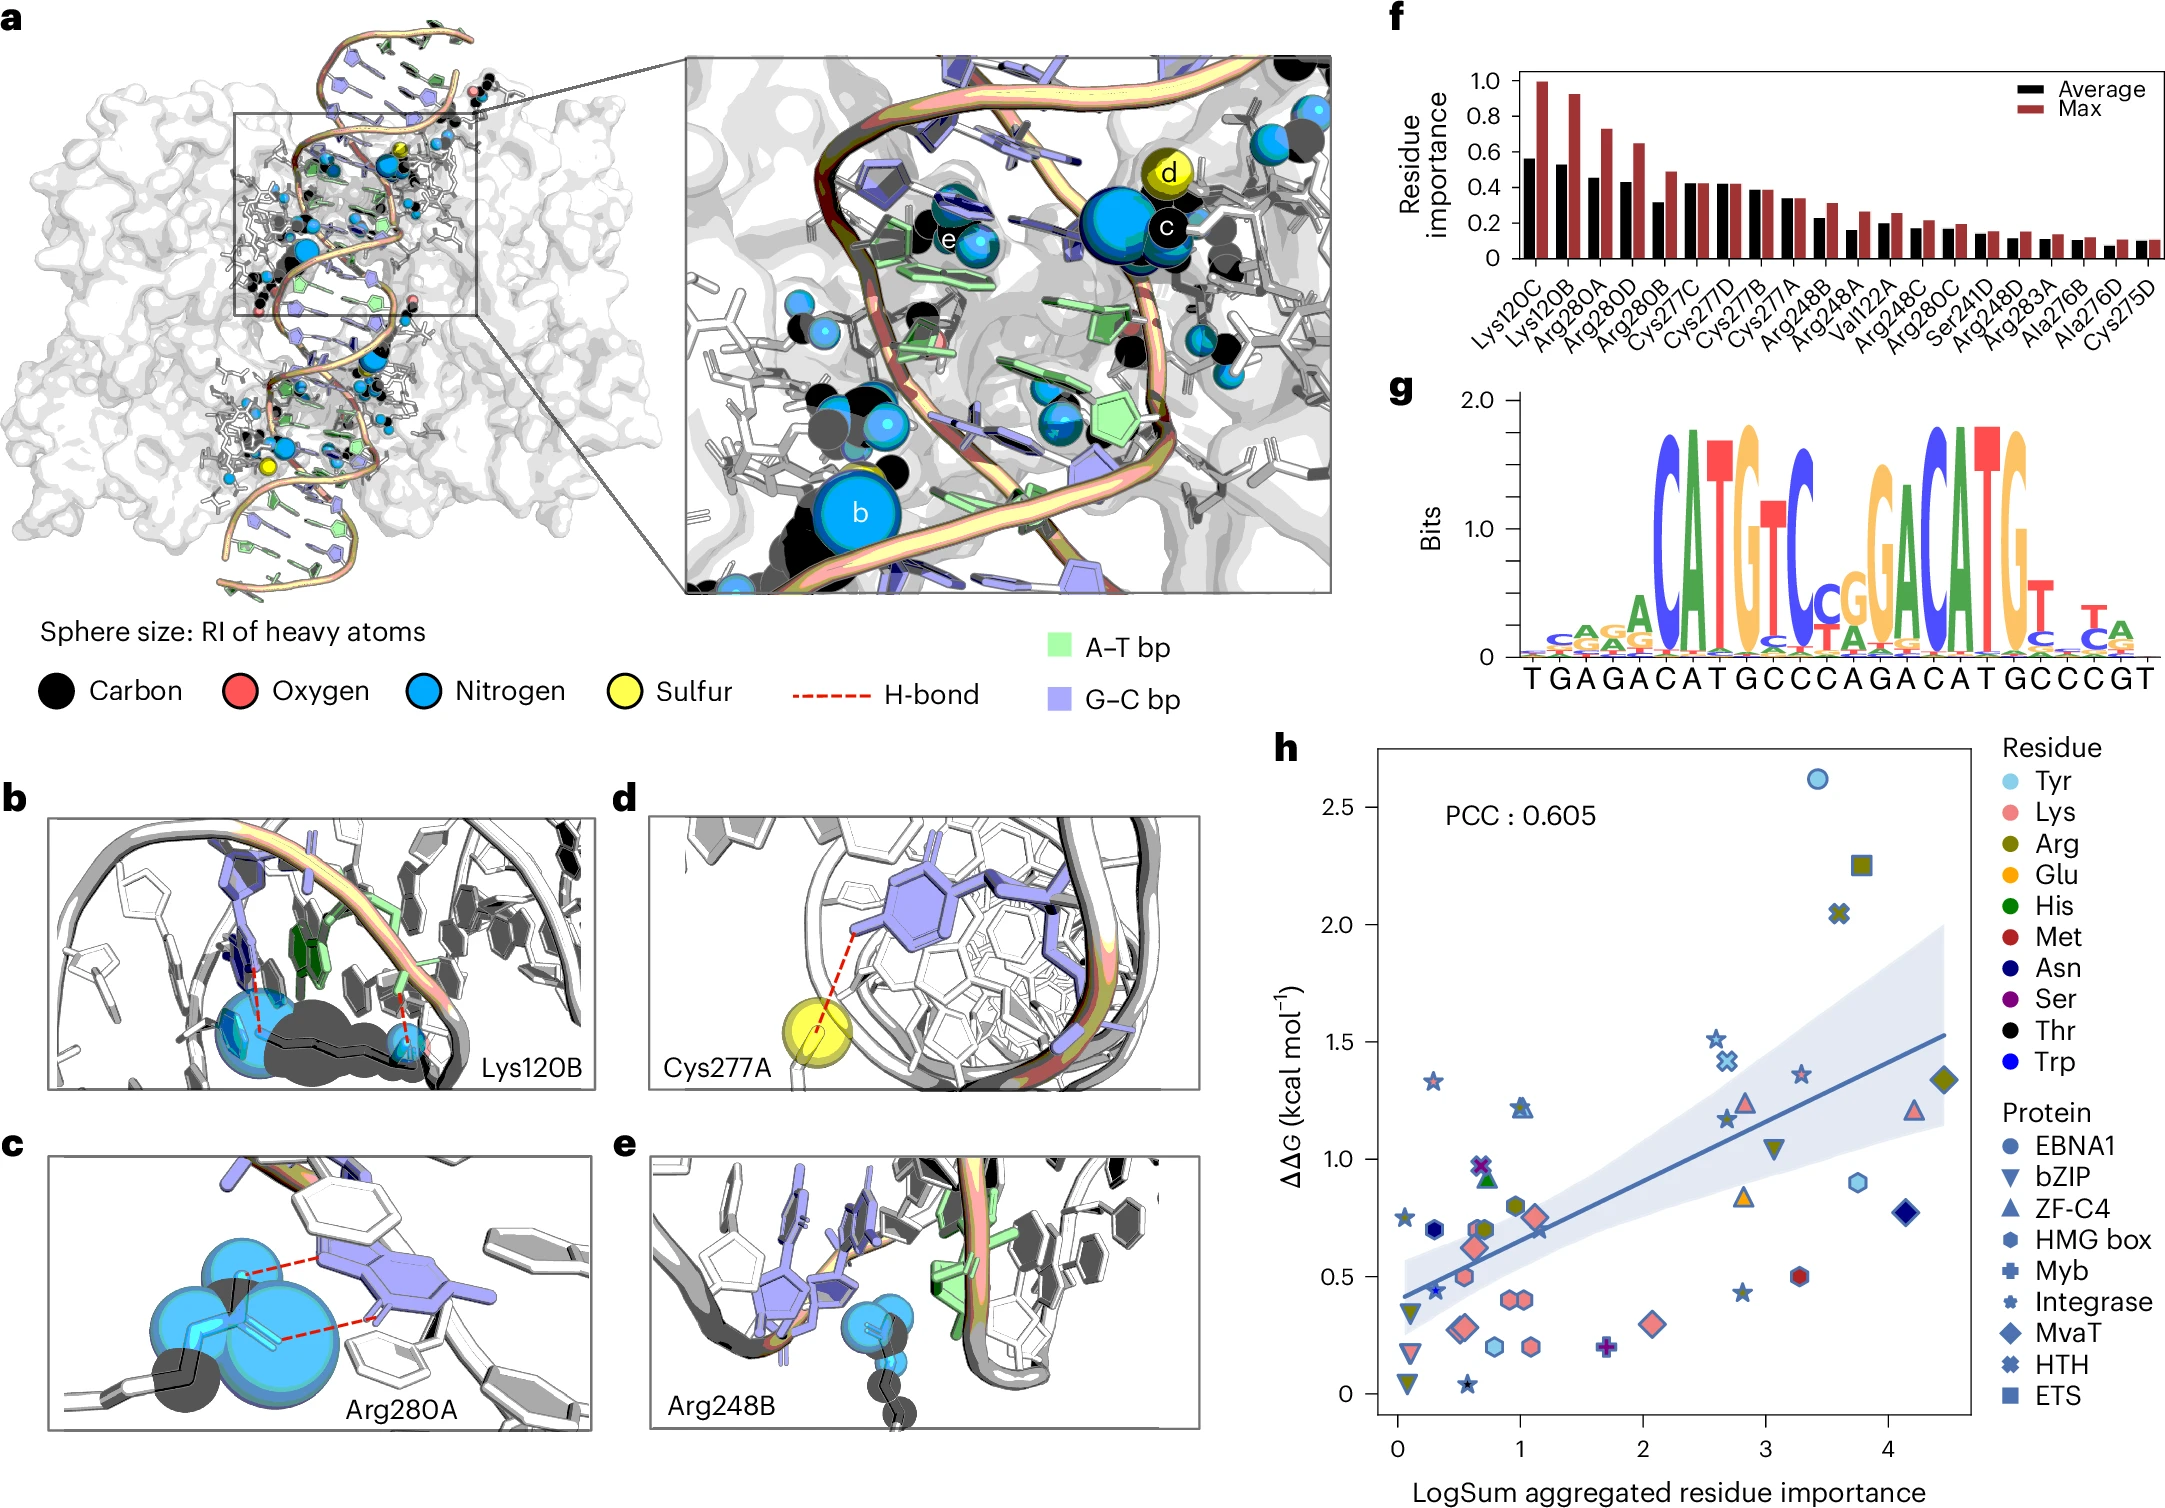
\includegraphics[width=0.8\paperwidth]{./pdnafigs/fig4.png}}
 % archetecture.png: 1149x508 px, 72dpi, 40.53x17.92 cm, bb=0 0 1149 508
        \caption[Computational cost of training RVAgene]{\textbf{Training RVAgene is reasonably scalable on CPU and even more so using hardware acceleration through GPU.} ({\bf A}) Time cost of training RVAgene for 100 epochs for datasets with varying number of genes and time points on CPU and GPU. ({\bf B}) Maximum memory utilized during training of the model on CPU an GPU for the cases in (A), inset plot: comparison of max memory used compared to DPGP for varying number of genes.}
  \label{fig:pdna4}
\end{figure}
\end{center}
\subsection{Application to designed scaffolds targeting specific DNA}
Recent work \citep{Glasscock2023} made significant progress in designing structural models of fully synthetic helix-turn-helix (HTH) protein scaffolds targeting specific DNA sequences. We applied DeepPBS to synthetically designed proteins targeting a specific DNA sequence (GCAGATCTGCACATC), named DBP5/6/9/35, respectively (Fig. 5a,e,i,m). The predicted PWMs are shown (Fig. 5b,f,j,n) and the heavy atom level RI scores are visualized for the interfaces (Fig. 5c,g,k,o). We explored qualitative agreement of these predictions with experimental results obtained from the study (Fig. 5d,h,l,p, relative binding signal of all possible single base-pair mutations obtained via flow cytometry analysis \citep{Glasscock2023} in yeast display competition assays). DeepPBS mostly correctly predicted the columns of high specificity (where the mutants show less binding that is darker red) except for a couple of cases. Some of the alternate base preference predictions by DeepPBS appear to agree with the experimental data. For example, for DBP35-position 11, DeepPBS predicts an alternate specific binding possibility to C along with the WT base A, and similarly for DBP35-position 9 and DBP5-position 7. Also, it is important to look at the flanking predictions for DeepPBS’ ability to produce sensible predictions for unbound DNA regions. For DBP9 and DBP6, the flanking predictions look remarkably uniform, which is consistent with the designed structure having mostly unbound canonical B-DNA structure. This baseline behavior is intuitive and nontrivial in this problem setting (given that there is a DNA sequence present in the design and the model has to circumvent overfitting of it). On the other hand, for DBP5 and DBP35, the flanks have a non-canonical shape with a narrow minor groove interaction with a loop region of the protein (obtained from PDB ID 1L3L). The DeepPBS prediction of a mostly A-tract preference (positions 3-8) is consistent with narrow minor groove preferred by such sequences \citep{Stefl2004}. DNA shape prediction \citep{Li2023} for the top base prediction of these columns (AAATTT) is consistent with the shape visualized in the design (Supplementary Fig. 12), showing a significant dip in minor groove width. These examples illustrate the potential for DeepPBS as a computational guide to performing expensive and laborious wet lab experiments.
\subsection{Application of DeepPBS to MD simulation of Exd-Scr–DNA system}

Owing to a fast inference time, DeepPBS can be used to analyze molecular simulation trajectories. We demonstrated how the protein heavy atom-level interpretability allows automatic detection of conformational changes in the protein-DNA interface. We applied DeepPBS to an MD simulation of the well-studied Exd-Scr-DNA system (Fig. S7a) (PDB ID: 2R5Z)\citep{Abe2015, Chiu2022, Ghoshdastidar2022, Slattery2011}. Details of the simulation method are provided in Supplementary Section 9. By computing the DeepPBS prediction over the trajectory, (Supplementary Video S1) consistent with the known binding specificity29 of the system. The
simulation trajectory was divided into 3,000 snapshots (0.1 ns apart), and the DeepPBS ensemble was applied to predict binding specificity for each snapshot. Relative importance (RI) scores were calculated for each heavy atom within 5 Å of DNA, followed by computation of max-aggregated residue RI scores. Fig. S6a shows the initial structure of the simulation, with the locations of some residues of interest marked. Residues Arg5 and His-12 of the Scr protein contribute to minor groove narrowing through electrostatic interactions, which play a crucial role in determining binding specificity \citep{Joshi2007}. 
Residues Arg58, Ile57, and Lys61 on the Exd protein interact with the major groove, driving specificity through hydrogen bonding and van der Waals interactions. In the simulation, residues Arg2, Arg3, and Arg5 on Exd contact with the flanking sequences. 

Variation of RI of the residues discussed earlier are shown in Fig. S6b,d,f. Supplementary Video 1 shows a concurrent view of changes in the network prediction as the simulation progressed, along with corresponding changes in the heavy atom RI score. Throughout the trajectory, Arg5 and His-12 on Scr consistently interact in the minor groove to drive protein-DNA binding specificity (Fig. S6e). Our model assigns stable RI scores to these residues (Fig. S6d). Arg58 strongly drives specificity by contacting G in the major groove, forming a bidentate hydrogen bond. However, after ~100 ns of simulation, the Exd recognition helix moves closer to the DNA major groove, leading to rotation of Arg58 (Fig. S6f, g) and causing a loss of strong specificity for G. Lys61 intermittently contacts the DNA through strong electrostatic interactions, leading to a gain in RI (Fig. S6f, g). 

RI scores assigned by our end-to-end deep-learning model offer an efficient alternative to traditional energy calculations, which require meticulous force-field design and energy computations. In the case of residues Arg2, Arg5, and Arg3 at the terminal loop region of the Exd protein, temporal changes in RI scores (Fig. S6b) strongly correspond to conformational changes of these residues over the simulation trajectory, as highlighted in Fig. S6c. Arg2 forms a bidentate hydrogen bond with G (~40 ns to 100 ns), which appears in DeepPBS predictions as highly specific for C (Fig. S6b). Arg5 interacts with an adjacent minor groove for most of the trajectory; however, it deviates away from the minor groove after ~210 ns, and a corresponding reduction in RI is observed. This demonstrates the ability of our deep-learning model to capture the dynamic behavior of residues and their interactions with the DNA.

DeepPBS has demonstrated its robustness and adaptability in response to both small dynamical fluctuations and conformational changes. Although the model was trained on snapshot structures and experimental PWMs, its predictions and RI scores are well-regularized and versatile, making it suitable for automated analysis of MD trajectories and designed protein-DNA complexes. These factors make DeepPBS a valuable tool for researchers working in the field of protein-DNA interactions, enabling deeper understanding and insights into the behavior of these complex molecular systems.

\subsection{Details on outliers seen on the benchmark set performance}

The outlier for the DeepPBS (Groove Readout) model is a TATA-box binding protein (TBP) bound to nucleosome bound-DNA (PDB ID: 7OH9). It is understandable that the ‘groove readout’ model will fail for this structure simply because TBP-DNA binding is known to be a primarily ‘shape readout’ driven process depending on the strong bendability and high conformational flexibility of the TATA motif \citep{simon2006}. Other than data quality limitations, another form of data limitation can be representation. For example, carboxylic acid side chains (glutamic and aspartic acids) are generally rare in biological DNA binding domains and hence in DeepPBS training data. A synthetic protein chemist should be weary of this fact, while designing domains with these residues. 

\begin{center}
    \begin{figure}
    \makebox[\textwidth]{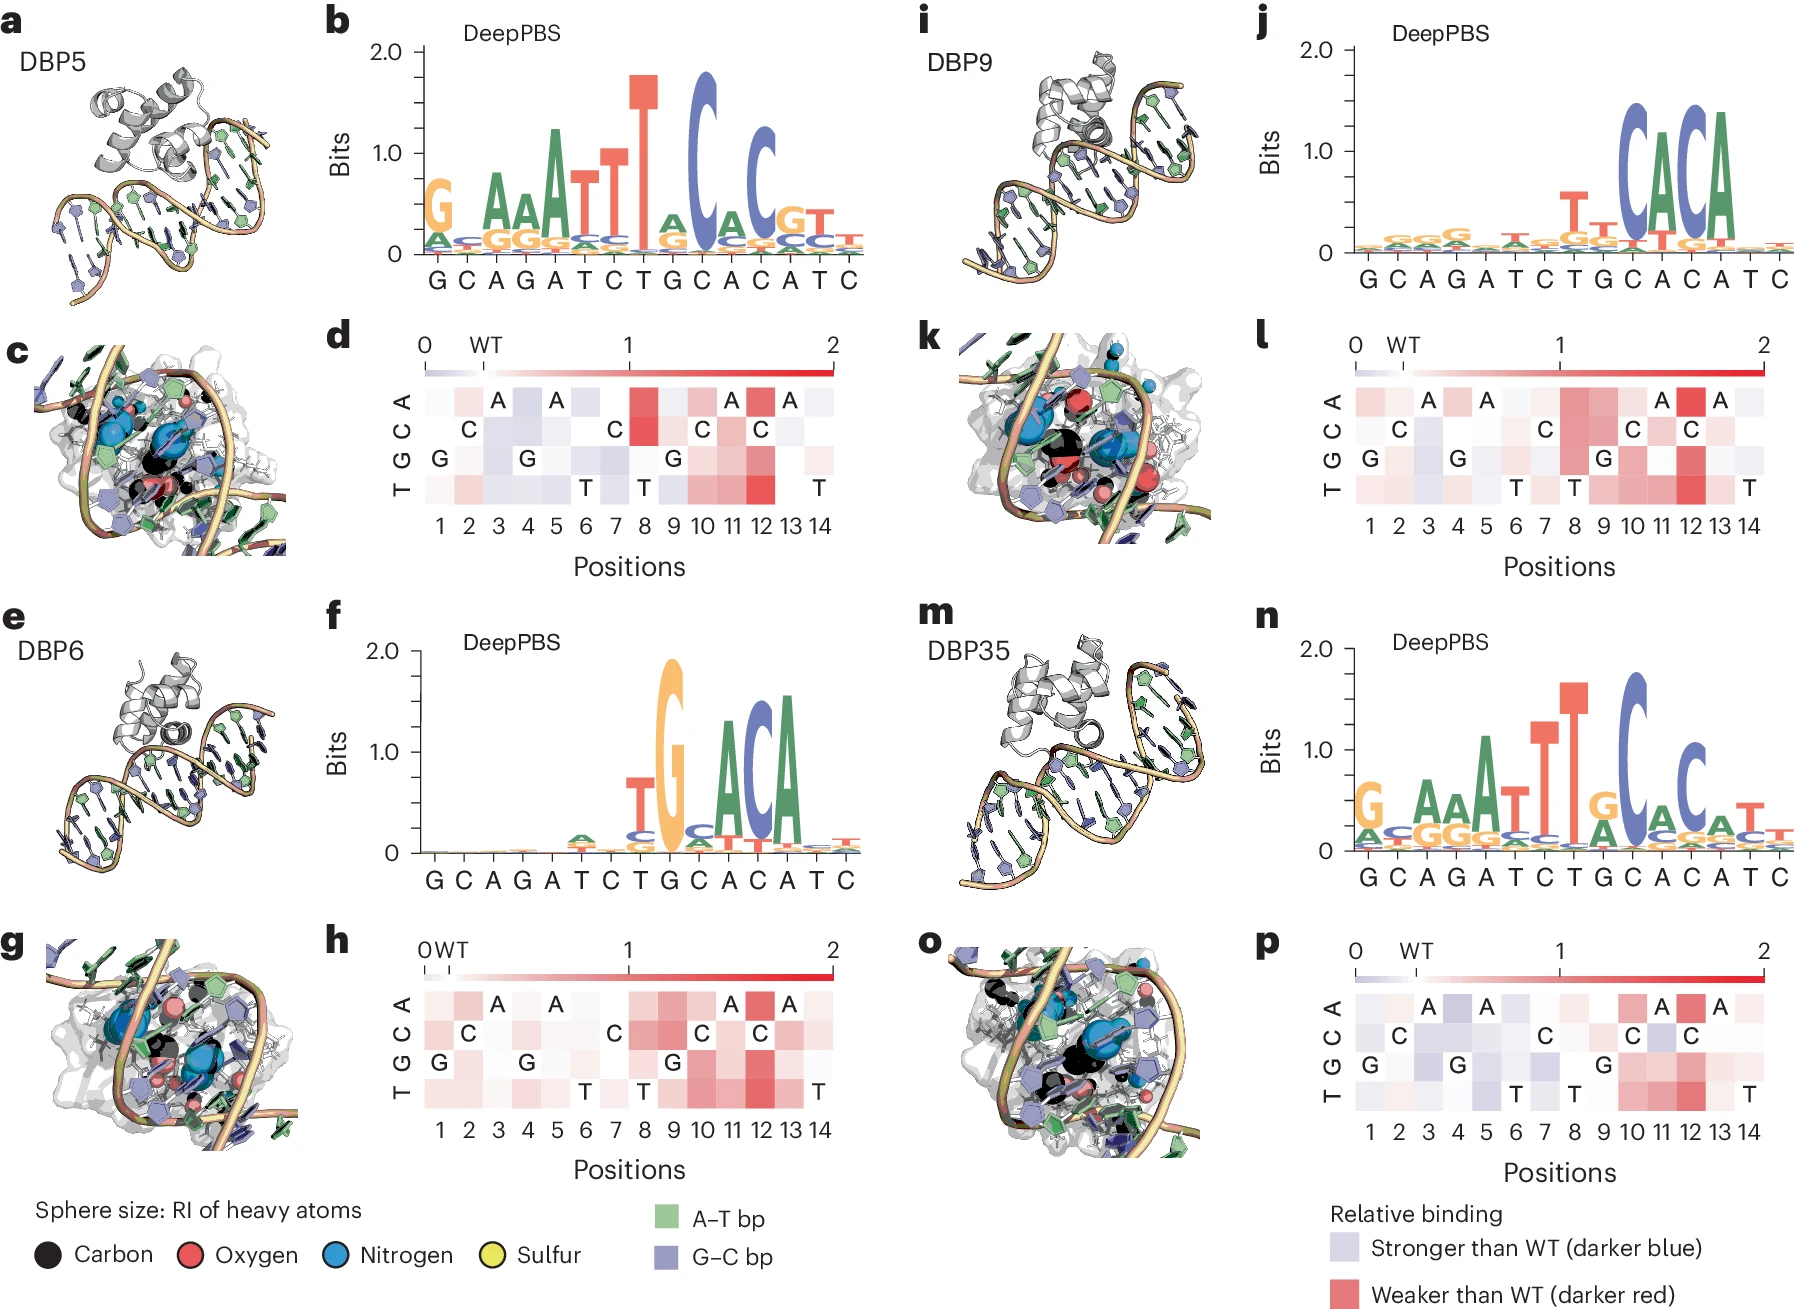
\includegraphics[width=0.8\paperwidth]{./pdnafigs/fig5.png}}
 % archetecture.png: 1149x508 px, 72dpi, 40.53x17.92 cm, bb=0 0 1149 508
        \caption[Computational cost of training RVAgene]{\textbf{Training RVAgene is reasonably scalable on CPU and even more so using hardware acceleration through GPU.} ({\bf A}) Time cost of training RVAgene for 100 epochs for datasets with varying number of genes and time points on CPU and GPU. ({\bf B}) Maximum memory utilized during training of the model on CPU an GPU for the cases in (A), inset plot: comparison of max memory used compared to DPGP for varying number of genes.}
  \label{fig:pdna5}
\end{figure}
\end{center}
